\documentclass{article}

% Official ICLR 2027 style files, as permitted by the Meta-Agents Workshop
% call for papers ("either the NeurIPS 2026 LaTeX template or the ICLR 2027
% LaTeX template"). Downloaded from:
%   https://media.iclr.cc/Conferences/ICLR2027/iclr-2027-style-files.zip
% \iclrfinalcopy is intentionally left commented out so the submission stays
% anonymous for double-blind review.
\usepackage{iclr2027_conference,times}

\usepackage[utf8]{inputenc}
\usepackage[T1]{fontenc}
\usepackage{hyperref}
\usepackage{url}
\usepackage{booktabs}
\usepackage{amsfonts}
\usepackage{amsmath}
\usepackage{graphicx}
\usepackage{xcolor}
\usepackage{microtype}
\usepackage{enumitem}
\usepackage{array}

\title{Selecting Worker-Agent Training Context \\ Under Continual Tool-Use Shift}

% Authors are omitted for double-blind review. Do not uncomment
% \iclrfinalcopy above until the camera-ready stage.
\author{Anonymous authors \\ Paper under double-blind review}

\begin{document}

\maketitle

\begin{abstract}
Meta-agents need reliable ways to train and evaluate the worker agents they manage. We ask whether a controller can select between two worker-agent training-context policies after each stage of a continual tool-use stream: A strips prior action--observation lines, while B retains them. The controller observes validation metrics only, candidate training is token-matched, and API families are partitioned disjointly into fit, controller-validation, and final-test roles. In a completed seed-42 run on the canonical stream order, the controller selected the trajectory policy B at all four stages, by validation-score margins of 0.08 to 0.14. On held-out test families the selected worker reaches 43.2\% exact full-call accuracy, 76.0\% API-name accuracy, and an 82.7\% valid-call rate. The controller's own validation traces reproduce the tradeoff that motivates the design: A almost never emits an unparseable call but selects the wrong API in 33--48\% of cases, while B cuts wrong-API errors to 2--7\% at the cost of 11--23\% malformed or absent calls. A supervisor optimizing aggregate exact match alone would not observe this exchange.
\end{abstract}

\section{Introduction}

A meta-agent that trains or improves another agent needs feedback about more than a final scalar score. For tool-use agents, an interaction exposes a structured action--observation history: the request made to an API, the returned observation, and the next action selected by the agent. These traces are externally auditable records of worker behavior, not private chain-of-thought.

We ask: \emph{under a fixed token budget, can a controller select between stripped-context and trajectory-context training for a continually adapting tool-use worker, using only validation signals, and does that selection generalize to unseen API families and stream orders?} This is a component-level instance of meta-agent post-training: the controller makes a policy decision about how another agent should learn.

The worker policies are A, which removes prior API request and response lines from the prompt, and B, which preserves them. Both predict the next API call; this is a context-policy comparison, not a pure final-response-only versus process-supervision comparison. API families are assigned to disjoint fit, controller-validation, and final-test partitions. After each stream stage, the controller trains both candidates from the currently selected adapter, evaluates them on validation families, and carries the higher-scoring adapter to the next stage. The final test families are not used for selection, score design, or stream-order tuning.

We also retain the earlier fixed-policy pilot as diagnostic evidence. It shows why a controller should use decomposed reliability metrics: B greatly reduces wrong-API errors but increases malformed/no-call outputs, and its original run receives 25.1\% more training tokens. The new protocol addresses the budget issue for candidate training and makes the meta-level decision auditable.

Our contributions are:
\begin{itemize}[leftmargin=*]
    \item A controller protocol that selects between two worker-agent training-context policies after each continual-learning stage using validation metrics only.
    \item A leakage-resistant evaluation design with disjoint API-family fit, controller-validation, and final-test partitions. The protocol also specifies held-out stream orders; only the canonical order was completed in the run reported here.
    \item A reliability-aware selection score that separates tool selection, exact arguments, valid-call rate, malformed/no-call behavior, and wrong-API behavior.
    \item An empirical result in which the controller selects the same policy at every stage, reported with its per-stage decision margins.
    \item A diagnostic fixed-policy comparison, corroborated by the controller's own validation traces, showing why meta-agents optimizing only aggregate exact match can select an unreliable worker policy.
\end{itemize}

The study is deliberately component-level. We do not claim to introduce a complete self-improving meta-agent, and we do not use private reasoning traces. We report one completed controller run, on the canonical stream order; the reverse and rotated orders defined by the protocol were not completed. The fixed-policy pilot is reported separately, and is not directly comparable to the controller numbers because it is scored on a different evaluation split.

\section{Related Work}

\paragraph{Tool-use agents and trajectories.}
Toolformer showed that language models can learn when and how to call external tools \citep{schick2023toolformer}, and ReAct established the interleaved reason-act-observe loop that produces the action--observation traces we study \citep{yao2023react}. API-Bank provides structured dialogues containing API requests, responses, and assistant actions \citep{li2023apibank}; ToolLLM and Gorilla scale tool-use supervision to substantially larger API collections \citep{qin2023toolllm,patil2023gorilla}. Broader agent benchmarks evaluate multi-turn task completion rather than single-call correctness \citep{liu2023agentbench,yao2024taubench}. Our setting uses API-Bank because its compact size permits repeated sequential fine-tuning and complete generation evaluation; the cost is that we score next-call prediction rather than end-to-end task success.

\paragraph{Meta-agents and automated optimization of agents.}
A growing body of work has one system improve another. Reflexion and Self-Refine feed a critique of an agent's output back into the same agent at inference time \citep{shinn2023reflexion,madaan2023selfrefine}, while STaR bootstraps training data from a model's own successful attempts \citep{zelikman2022star}. A second line optimizes the artifacts around a model rather than its weights: OPRO uses a language model as the optimizer of its own prompts \citep{yang2023opro}, DSPy compiles declarative pipelines and tunes their modules \citep{khattab2023dspy}, and TextGrad propagates textual feedback through a computation graph \citep{yuksekgonul2024textgrad}. Closest to our framing, ADAS searches over agent designs themselves \citep{hu2024adas}, and AutoGen provides the multi-agent substrate such systems are typically built on \citep{wu2023autogen}. Our controller is far narrower than any of these: it optimizes neither prompts nor architecture but the training context supplied to a worker, over a two-element candidate set, and it makes its decisions from held-out validation metrics rather than from model self-assessment.

\paragraph{Process and outcome supervision.}
Process supervision can outperform final-answer supervision in mathematical reasoning \citep{lightman2023verify,uesato2022process}, and later work reduces its labeling cost by inferring step-level rewards automatically \citep{wang2023shepherd}. API trajectories are a narrower signal: they record observable interaction events rather than internal reasoning steps or human labels. We therefore use the term trajectory context and avoid treating API traces as faithful representations of thought. The reliability of automatic scoring is itself contested \citep{zheng2023judging}, which is part of why our controller scores decomposed, parser-level outcomes rather than a single learned judgment.

\paragraph{Continual learning.}
Sequential fine-tuning degrades earlier capabilities, a failure documented long before language models \citep{kirkpatrick2017overcoming,lopezpaz2017gem} and confirmed for large-scale instruction tuning \citep{luo2023empirical}. This motivates evaluation protocols that measure adaptation and forgetting jointly \citep{wang2023trace}, which our evaluation matrix follows, and mitigation methods that constrain where adaptation happens \citep{wang2023olora}. Efficient adaptation methods such as LoRA and QLoRA make it practical to train multiple worker-agent variants \citep{hu2021lora,dettmers2023qlora}.

\paragraph{Selecting between candidates under a noisy signal.}
Choosing among partially trained candidates on limited validation evidence is a well-studied problem outside the agent literature. Hyperband allocates budget to candidates by successive elimination \citep{li2018hyperband}, and population-based training interleaves selection with continued training in a way structurally similar to our stage-wise loop \citep{jaderberg2017pbt}. Both treat the number of validation samples backing a decision as a first-class quantity. Our controller is a deliberately simple instance of this family, and Section~\ref{sec:limitations} reports the validation sample sizes its decisions actually rest on.

\section{Worker-Agent Setup}
\label{sec:setup}

\subsection{Task and stream construction}

We use API-Bank, a dataset of tool-augmented dialogues, and construct four sequential blocks $D_1,\ldots,D_4$ by grouping examples by API family. The blocks are disjoint in their assigned examples. Within each block, API families are deterministically assigned to fit, controller-validation, or final-test roles. Fit uses only original training examples; validation and test use only original held-out examples, and no API family appears in more than one role. The protocol defines canonical, reverse, and one-block-rotated stream orders; the run reported in this paper completed the canonical order only. At each stage the controller trains candidates on fit families and observes validation metrics only. Final test-family evaluation occurs after all selections and is never used for score design or policy selection.  The controller's validation history is stage-indexed, recording stage-wise validation metrics rather than producing a $4 \times 4$ matrix. Rows index the training stage and columns index the evaluation block.

The primary generation task is next-API-call prediction. We score examples whose expected output contains a parseable API call. The full held-out evaluation contains 126, 104, 103, and 107 scored examples in $D_1$ through $D_4$, respectively. The training notebook also reports a sampled evaluation of 32 examples per block at each stage; we report it separately because it is useful for continual-learning metrics but has higher sampling noise.

\subsection{Training conditions and controller}

The stripped-context condition, A, removes previous lines beginning with \texttt{API-Request:} or \texttt{API-Response:}, as well as the corresponding trace markers, before training and generation evaluation. It is a stripped-context next-call baseline, not a pure final-response-only condition: both conditions predict the next API call when the target is an API call.

The trajectory condition, B, retains the previous API requests and responses in the prompt. Generation evaluation uses the same condition-specific format as training. This alignment matters: evaluating B with stripped prompts would create a train/test mismatch and confound the comparison.

At stage $t$, both candidate adapters $W_t^A$ and $W_t^B$ are trained from the previously selected adapter $W_{t-1}$ on the current block's fit families. The controller evaluates each candidate on validation families from blocks observed through stage $t$ and selects $W_t=\arg\max_{c\in\{A,B\}}S(V_t^c)$. The score is frozen before testing:
\[
S(V)=0.50a_{\mathrm{exact}}+0.20a_{\mathrm{name}}+0.20r_{\mathrm{valid}}-0.05r_{\mathrm{malformed}}-0.05r_{\mathrm{wrong\mbox{-}API}}.
\]
Candidate training is token-matched by capping B to the number of truncated training tokens used by A for the same fit families. The controller's decision history, candidate scores, and selected adapter are saved for audit.
All runs use \texttt{meta-llama/Llama-3.1-8B-Instruct}. We use QLoRA with 4-bit NF4 quantization, LoRA rank 32, alpha 64, bfloat16 computation, maximum sequence length 1024, effective batch size 16, learning rate $2 \times 10^{-4}$, and three epochs per block. The recorded run uses seed 42. The A run used an NVIDIA RTX PRO 6000 Blackwell Server Edition and the B run used an NVIDIA H100 80GB; both have sufficient memory for the configuration.

The earlier fixed-policy pilot was not token-budget matched: A consumed 1,857,169 training tokens and B consumed 2,324,314, so B received 25.1\% more tokens. The controller experiment uses token-matched candidate training; we report the pilot separately from controller results.

\subsection{Metrics}

For each generated call, we parse the API name and single-quoted parameter assignments, then normalize names and parameter strings for comparison. We report:

\begin{itemize}[leftmargin=*]
    \item \textbf{API-name accuracy}: the generated API name matches the expected name.
    \item \textbf{Exact full-call accuracy}: the API name and normalized parameter dictionary match exactly.
    \item \textbf{Name plus any parameter}: the API name and at least one expected parameter-value pair match.
    \item \textbf{Malformed/no-call rate}: no parseable API call is generated.
\end{itemize}

For the sampled continual-learning matrix, we also calculate final average accuracy (AA), backward transfer (BWT), forward transfer (FWT), average forgetting, and area under the learning curve (AULC). These metrics are descriptive for this one seed; they are not accompanied by uncertainty estimates.

\section{Results}
\label{sec:pilot}

\subsection{Full held-out generation}

Table~\ref{tab:final} reports the final-stage results after training through $D_4$. B improves exact full-call accuracy on every held-out block, with a mean increase of 17.7 percentage points. The gain in API-name accuracy is smaller but consistent in the mean, at 7.7 points. Name-plus-any-parameter accuracy also improves on every block. Figure~\ref{fig:heatmaps} shows the same comparison as stage-by-block matrices, where the advantage holds at every training stage rather than only at the end of the stream.

\begin{table}[t]
\centering
\caption{Full held-out generation results after sequential training through $D_4$. Values are percentages.}
\label{tab:final}
\resizebox{\linewidth}{!}{%
\begin{tabular}{llrrrrr}
\toprule
Condition & Metric & D1 & D2 & D3 & D4 & Mean \\
\midrule
A & Exact full call & 35.7 & 43.3 & 32.0 & 45.8 & 39.2 \\
B & Exact full call & 57.9 & 61.5 & 44.7 & 63.6 & 56.9 \\
\midrule
A & API name & 64.3 & 62.5 & 60.2 & 79.4 & 66.6 \\
B & API name & 73.8 & 82.7 & 67.0 & 73.8 & 74.3 \\
\midrule
A & Name + any parameter & 51.6 & 56.7 & 50.5 & 65.4 & 56.1 \\
B & Name + any parameter & 67.5 & 76.9 & 61.2 & 72.0 & 69.4 \\
\bottomrule
\end{tabular}}
\end{table}

\begin{figure}[t]
\centering
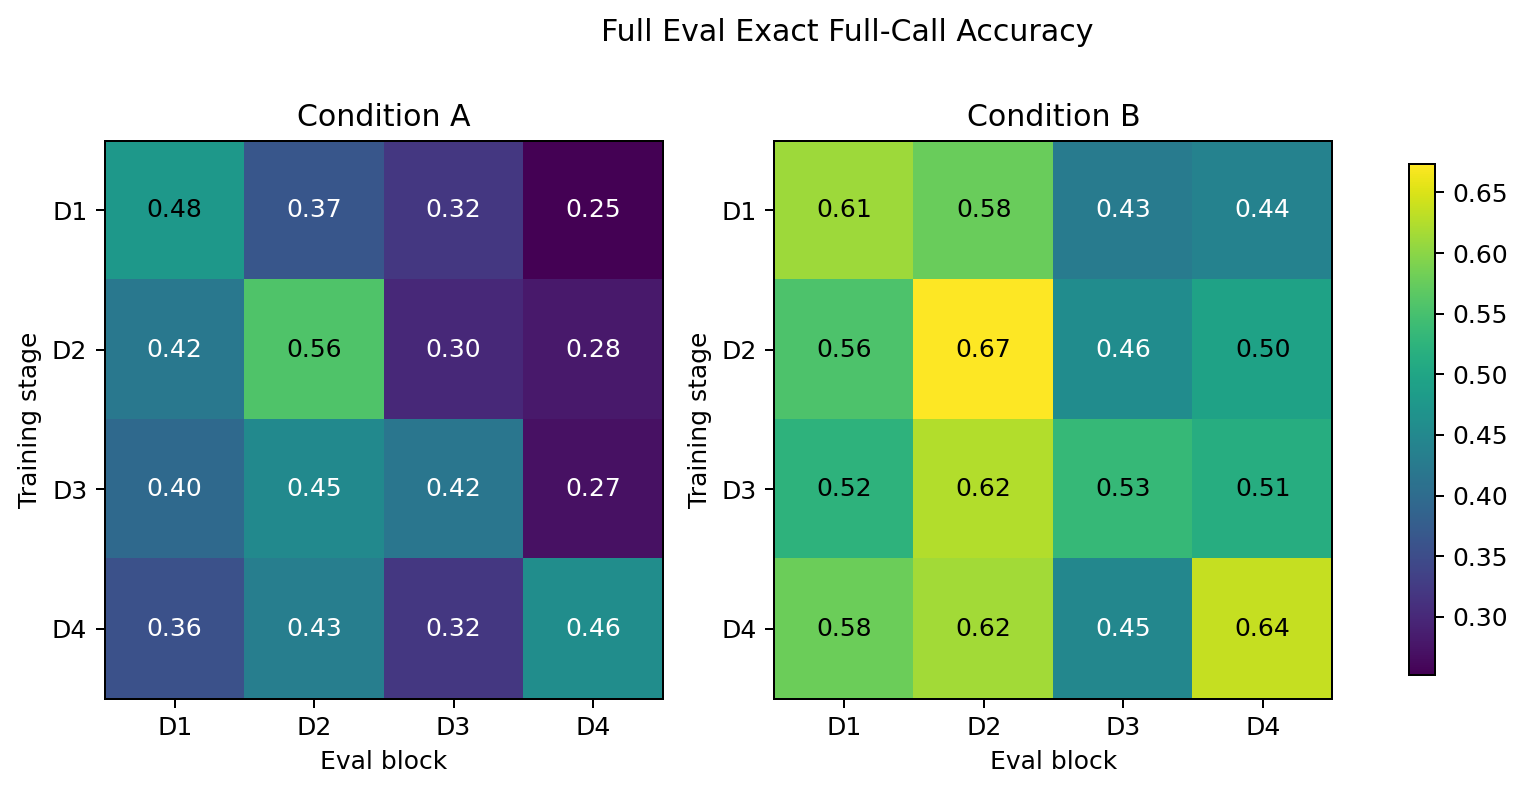
\includegraphics[width=0.91\linewidth]{figures/full_eval_exact_full_heatmaps_seed42.png}
\caption{Full held-out exact full-call accuracy matrices. Rows are training stages and columns are evaluation blocks. The trajectory condition is higher on every final-stage block, while earlier-block performance still changes over the stream.}
\label{fig:heatmaps}
\end{figure}

\subsection{Continual-learning behavior}

The sampled evaluation gives final AA of 38.3\% for A and 53.9\% for B. B also has higher FWT (33.3\% versus 22.9\%) and higher AULC (57.2\% versus 41.8\%). These results are consistent with faster or stronger adaptation to the stream, although they are measured on a small fixed sample and B receives more tokens.

The forgetting metrics point in the opposite direction. BWT is $-13.5\%$ for B and $-10.4\%$ for A, while average forgetting is 13.5\% for B and 10.4\% for A. Thus, the trajectory condition should not be described as reducing forgetting in this experiment. The more accurate conclusion is that it improves final accuracy and forward transfer while not improving, and possibly worsening, the measured retention tradeoff. Figure~\ref{fig:sampled} summarises both sides of this comparison.

\begin{figure}[t]
\centering
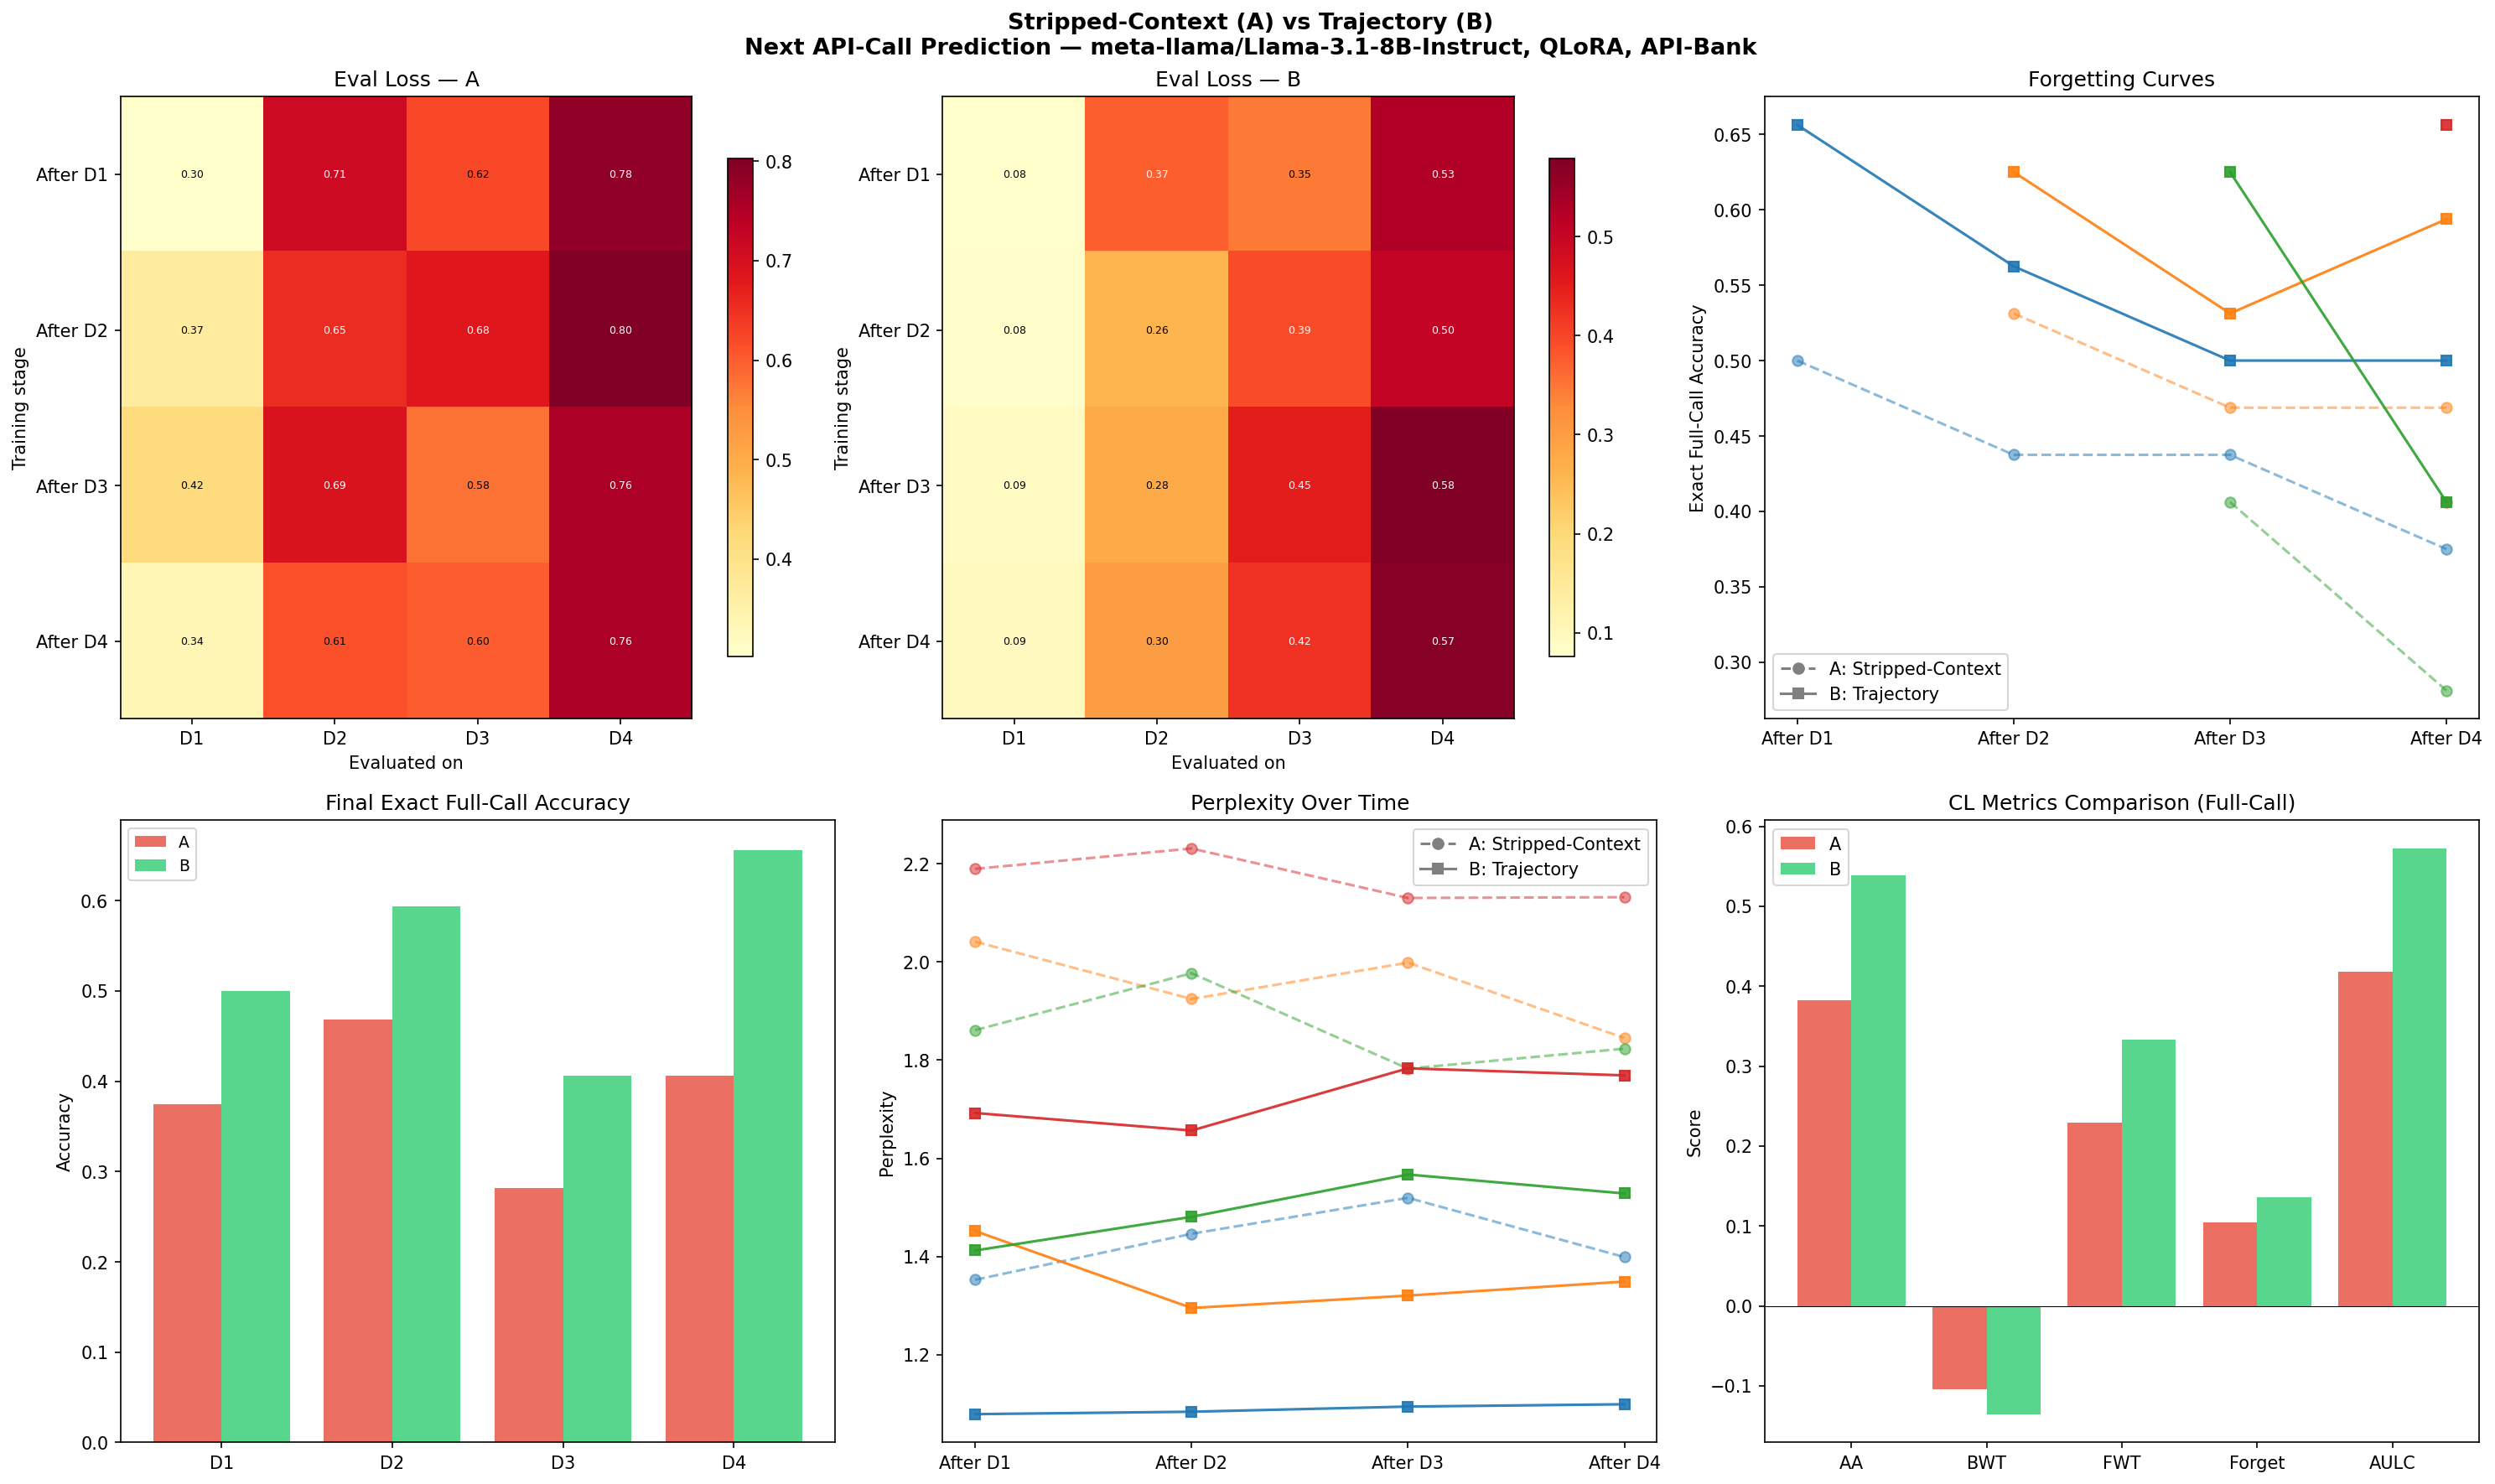
\includegraphics[width=0.91\linewidth]{figures/sampled_eval_summary.png}
\caption{Sampled continual-learning evaluation. B has higher final average accuracy and forward transfer, but both conditions show forgetting and B's sampled retention metrics are more negative.}
\label{fig:sampled}
\end{figure}

\subsection{Failure modes}
\label{sec:failuremodes}

The aggregate gain is driven partly by tool selection. Across all final-stage scored examples, A produces 102 wrong-API errors and B produces 12. B also reduces correct-API/wrong-parameter errors from 47 to 22. However, B produces 101 malformed or no-call outputs versus 45 for A. Table~\ref{tab:errors} gives the full breakdown. This means a supervisor using only exact-call accuracy could miss a reliability regression in output formatting or call emission.

\begin{table}[t]
\centering
\caption{Final-stage error categories across all scored blocks. Counts are mutually exclusive under the evaluation parser.}
\label{tab:errors}
\begin{tabular}{lrr}
\toprule
Category & A & B \\
\midrule
Exact full call & 172 & 251 \\
Correct API, some parameters & 74 & 54 \\
Correct API, wrong parameters & 47 & 22 \\
Wrong API & 102 & 12 \\
Malformed or no call & 45 & 101 \\
\bottomrule
\end{tabular}
\end{table}

For a meta-agent, this decomposition is operationally important. A controller that optimizes only exact-match reward could prefer a policy that selects the right tool more often but emits more invalid actions. Any automatic optimizer should therefore use multiple constraints or reward terms, including parse validity, semantic argument correctness, and task completion.

\section{Controller Results}

We report one completed controller run: seed 42, \texttt{meta-llama/Llama-3.1-8B-Instruct}, token-matched candidate training, canonical stream order. The run comprises 12 QLoRA trainings (eight for controller fitting, four for the frozen-schedule replay) and 1.95 GPU-hours. The recorded split assigns 115 API families to fit, 32 to controller validation, and 37 to final test, with no family in more than one role.

\subsection{The selection loop is degenerate}

Table~\ref{tab:decisions} gives every controller decision. The trajectory policy B wins at all four stages, by margins of 0.078 to 0.135 on a score whose observed range across candidates is roughly 0.37 to 0.61. The controller therefore never switches, and on this stream it is behaviorally indistinguishable from a fixed B policy.

\begin{table}[t]
\centering
\caption{Controller decisions on the canonical order. $S$ is the frozen reliability-aware score, computed on controller-validation families only. The controller selected B at every stage.}
\label{tab:decisions}
\begin{tabular}{llrrrl}
\toprule
Stage & Block & $S(A)$ & $S(B)$ & Margin & Selected \\
\midrule
1 & $D_1$ & 0.491 & 0.605 & 0.114 & B \\
2 & $D_2$ & 0.463 & 0.586 & 0.123 & B \\
3 & $D_3$ & 0.375 & 0.510 & 0.135 & B \\
4 & $D_4$ & 0.379 & 0.457 & 0.078 & B \\
\bottomrule
\end{tabular}
\end{table}

Both candidate scores decline monotonically across stages, from 0.605 to 0.457 for B and from 0.491 to 0.379 for A.

\subsection{Held-out family evaluation}

Table~\ref{tab:controllerfinal} reports the selected worker on final-test families, which are disjoint from every family used for fitting or for controller validation. These numbers are not comparable to the fixed-policy pilot in Section~\ref{sec:pilot}: the pilot is scored on the full held-out split of each block, whereas the controller is scored only on the held-out test families, a smaller and family-disjoint set of 118 examples.

\begin{table}[t]
\centering
\caption{Selected worker on held-out test families, canonical order, evaluated under condition B. Values are percentages; $n$ is the number of scored examples.}
\label{tab:controllerfinal}
\begin{tabular}{lrrrrrr}
\toprule
Block & $n$ & Exact full call & API name & Valid & Malformed & Wrong API \\
\midrule
$D_1$ & 23 & 39.1 & 78.3 & 78.3 & 21.7 & 0.0 \\
$D_2$ & 28 & 46.4 & 82.1 & 92.9 & 7.1 & 10.7 \\
$D_3$ & 30 & 33.3 & 60.0 & 73.3 & 26.7 & 13.3 \\
$D_4$ & 37 & 54.1 & 83.8 & 86.5 & 13.5 & 2.7 \\
\midrule
Mean & & 43.2 & 76.0 & 82.7 & 17.3 & 6.7 \\
Pooled & 118 & 44.1 & 76.3 & 83.1 & 16.9 & 6.8 \\
\bottomrule
\end{tabular}
\end{table}

Pooling the 118 scored examples, the mutually exclusive outcome categories are 52 exact full calls, 38 correct-API calls with wrong parameters, 8 wrong-API calls, and 20 malformed or absent calls. Argument construction, not tool choice, is the dominant remaining error: the selected worker names the right API in 76.3\% of cases but gets the complete call right in 44.1\%.

\subsection{The controller reproduces the failure-mode tradeoff}

The controller's validation traces are an independent replication of the diagnostic in Section~\ref{sec:failuremodes}, now under token-matched training and with families disjoint from the test set. Table~\ref{tab:valtradeoff} shows the exchange at every stage: A is almost perfectly well-formed, emitting an unparseable call at most 3.5\% of the time, but selects the wrong API in 33 to 48\% of cases. B reduces wrong-API errors to between 2 and 7\% and pays for it with malformed or absent calls between 11 and 23\%.

\begin{table}[t]
\centering
\caption{Controller-validation aggregates by stage. A is reliably well-formed but frequently selects the wrong tool; B reverses the pattern. Values are percentages.}
\label{tab:valtradeoff}
\begin{tabular}{lrrrrrr}
\toprule
& \multicolumn{2}{c}{Exact full call} & \multicolumn{2}{c}{Malformed/no call} & \multicolumn{2}{c}{Wrong API} \\
\cmidrule(lr){2-3}\cmidrule(lr){4-5}\cmidrule(lr){6-7}
Stage & A & B & A & B & A & B \\
\midrule
1 & 36.4 & 63.6 & 0.0 & 22.7 & 36.4 & 4.5 \\
2 & 28.8 & 48.5 & 0.0 & 11.4 & 32.6 & 2.3 \\
3 & 19.3 & 36.2 & 2.1 & 13.8 & 45.1 & 3.6 \\
4 & 23.2 & 33.7 & 3.5 & 21.1 & 48.3 & 6.5 \\
\bottomrule
\end{tabular}
\end{table}

The two policies do not differ by a single quality scalar; they fail in different places. A meta-agent that reads only aggregate exact match would record B as uniformly better and would not observe that it has traded tool-selection errors for output-validity errors.

\section{Implications for Meta-Agent Systems}

The implemented experiment instantiates a narrow meta-agent: a controller that trains, evaluates, and selects a worker adapter. At each stage it compares A and B from the same parent adapter, observes validation metrics, and selects the candidate carried to the next stage. Its final evaluation is restricted to API families held out from both fitting and controller validation.

It uses a frozen score containing exact-call accuracy, API-name accuracy, valid-call rate, malformed/no-call rate, and wrong-API rate. The saved history exposes each candidate score and selected policy, making the decision auditable without exposing final-test metrics.

The fixed-policy pilot suggests that a useful controller objective should not be a single exact-call metric. The trajectory condition's reduction in wrong-tool errors is valuable, but its malformed/no-call increase is a warning that optimizing one observable metric can move failures elsewhere. The controller therefore uses a frozen multi-metric score.

We therefore report the selection rate and the per-stage decision margins alongside the selected schedule, since the schedule alone records only that B was chosen four times.

\section{Limitations}
\label{sec:limitations}

\paragraph{Incomplete stream-order evaluation.}
The protocol specifies canonical, reverse, and one-block-rotated stream orders, but only the canonical order was completed. The paper therefore contains no evidence about whether the selected schedule transfers to a different block ordering, and the stream-order component of our research question is unanswered.

\paragraph{Degenerate schedule.}
The controller made four decisions and they were identical, so this run provides no evidence that the selection mechanism can adapt, only that it prefers B consistently and by a clear margin.

\paragraph{Validation sample sizes.}
Controller decisions rest on 22, 28, 44, and 70 scored validation examples at stages 1 through 4. Block $D_2$ contributes only 6 scored examples through its 3 validation families. Stage-level decisions are correspondingly noisy.

\paragraph{Token budget and seed.}
Candidate training in the controller run is token-matched, but the fixed-policy pilot is not: there B receives 25.1\% more training tokens. The pilot's advantage may therefore reflect token quantity, trajectory content, or their interaction. Both the pilot and the controller run use only seed 42, and no confidence intervals or significance tests are reported for either.

\paragraph{Task and data scope.}
API-Bank is compact and structured, which supports controlled iteration but limits external validity. Four blocks are a short continual-learning stream. The task is next-call prediction rather than complete end-to-end task success.

\paragraph{Metric brittleness.}
Exact parameter matching and regular-expression parsing can classify semantically equivalent calls as failures. Conversely, API-name correctness does not guarantee a useful or safe action. Future evaluations should include semantic argument scoring and executable task-level outcomes.

\paragraph{Scope of meta-agent.}
The controller is deliberately narrow: it selects between two human-designed context policies and does not perform open-ended architecture search, self-rewriting, multi-agent delegation, or human management. Its contribution is an auditable post-training and evaluation component, not unrestricted self-improvement.

\section{Responsible-Use Statement}

Tool-use post-training can increase an agent's ability to select and invoke external APIs, so improvements should not be treated as permission to grant unrestricted access. The trajectories studied here are observable interaction records, not private reasoning, but they may still contain sensitive user or tool-output data; deployments should minimize collection, remove unnecessary identifiers, and apply access controls. Any meta-agent that trains or selects worker policies should operate in a sandbox with least-privilege tools, explicit human approval for consequential actions, complete audit logs, rate limits, and a rollback or halt mechanism. Evaluation should separately monitor invalid calls, unsafe tool selection, semantic argument errors, and metric gaming rather than optimizing exact-match accuracy alone. We recommend that future trajectory-optimization studies release only permitted, de-identified data and document dataset licenses and model-use restrictions.

\section{Conclusion}

We introduced a narrow meta-controller that selects between stripped-context and trajectory-context training for a continually adapting tool-use worker, and reported one completed seed-42 run on the canonical stream order. The controller selected the trajectory policy at all four stages. On held-out API families the selected worker reached 43.2\% exact full-call accuracy with a 17.3\% malformed rate.

Under token-matched training and disjoint family partitions, the controller's validation traces reproduce the pilot's finding that the two policies fail in different places: stripped context yields well-formed calls to the wrong tool, trajectory context yields the right tool with a higher rate of unparseable output. A meta-agent scoring only aggregate exact match cannot see that exchange, and would silently accept a reliability regression as an improvement.

The claim remains component-level. This run does not establish open-ended self-improvement, nor selection generalization: the reverse and rotated stream orders were not completed, the candidate set holds two human-designed policies, and everything rests on a single seed. Multiple seeds, the remaining stream orders, larger candidate sets, semantic argument scoring, and comparisons against learned or human-designed controller baselines are all needed before selection-based post-training can be claimed to work.

\small
\begin{thebibliography}{99}

\bibitem[Dettmers et al.(2023)]{dettmers2023qlora}
Tim Dettmers, Artidoro Pagnoni, Ari Holtzman, and Luke Zettlemoyer.
\newblock QLoRA: Efficient finetuning of quantized LLMs.
\newblock \emph{NeurIPS}, 2023.

\bibitem[Hu et al.(2022)]{hu2021lora}
Edward J. Hu, Yelong Shen, Phillip Wallis, Zeyuan Allen-Zhu, Yuanzhi Li, Shean Wang, Lu Wang, and Weizhu Chen.
\newblock LoRA: Low-rank adaptation of large language models.
\newblock \emph{ICLR}, 2022.

\bibitem[Hu et al.(2024)]{hu2024adas}
Shengran Hu, Cong Lu, and Jeff Clune.
\newblock Automated design of agentic systems.
\newblock \emph{arXiv:2408.08435}, 2024.

\bibitem[Jaderberg et al.(2017)]{jaderberg2017pbt}
Max Jaderberg, Valentin Dalibard, Simon Osindero, Wojciech M. Czarnecki, Jeff Donahue, Ali Razavi, Oriol Vinyals, Tim Green, Iain Dunning, Karen Simonyan, Chrisantha Fernando, and Koray Kavukcuoglu.
\newblock Population based training of neural networks.
\newblock \emph{arXiv:1711.09846}, 2017.

\bibitem[Khattab et al.(2023)]{khattab2023dspy}
Omar Khattab, Arnav Singhvi, Paridhi Maheshwari, Zhiyuan Zhang, Keshav Santhanam, Sri Vardhamanan, Saiful Haq, Ashutosh Sharma, Thomas T. Joshi, Hanna Moazam, Heather Miller, Matei Zaharia, and Christopher Potts.
\newblock DSPy: Compiling declarative language model calls into self-improving pipelines.
\newblock \emph{arXiv:2310.03714}, 2023.

\bibitem[Kirkpatrick et al.(2017)]{kirkpatrick2017overcoming}
James Kirkpatrick, Razvan Pascanu, Neil Rabinowitz, Joel Veness, Guillaume Desjardins, Andrei A. Rusu, Kieran Milan, John Quan, Tiago Ramalho, Agnieszka Grabska-Barwinska, Demis Hassabis, Claudia Clopath, Dharshan Kumaran, and Raia Hadsell.
\newblock Overcoming catastrophic forgetting in neural networks.
\newblock \emph{PNAS}, 114(13):3521--3526, 2017.

\bibitem[Li et al.(2018)]{li2018hyperband}
Lisha Li, Kevin Jamieson, Giulia DeSalvo, Afshin Rostamizadeh, and Ameet Talwalkar.
\newblock Hyperband: A novel bandit-based approach to hyperparameter optimization.
\newblock \emph{JMLR}, 18(185):1--52, 2018.

\bibitem[Li et al.(2023)]{li2023apibank}
Minghao Li, Yingxiu Zhao, Bowen Yu, Feifan Song, Hangyu Li, Haiyang Yu, Zhoujun Li, Fei Huang, and Yongbin Li.
\newblock API-Bank: A comprehensive benchmark for tool-augmented LLMs.
\newblock \emph{EMNLP}, 2023.

\bibitem[Lightman et al.(2023)]{lightman2023verify}
Hunter Lightman, Vineet Kosaraju, Yura Burda, Harri Edwards, Bowen Baker, Teddy Lee, Jan Leike, John Schulman, Ilya Sutskever, and Karl Cobbe.
\newblock Let's verify step by step.
\newblock \emph{arXiv:2305.20050}, 2023.

\bibitem[Liu et al.(2023)]{liu2023agentbench}
Xiao Liu, Hao Yu, Hanchen Zhang, Yifan Xu, Xuanyu Lei, Hanyu Lai, Yu Gu, Hangliang Ding, Kaiwen Men, Kejuan Yang, Shudan Zhang, Xiang Deng, Aohan Zeng, Zhengxiao Du, Chenhui Zhang, Sheng Shen, Tianjun Zhang, Yu Su, Huan Sun, Minlie Huang, Yuxiao Dong, and Jie Tang.
\newblock AgentBench: Evaluating LLMs as agents.
\newblock \emph{arXiv:2308.03688}, 2023.

\bibitem[Lopez-Paz and Ranzato(2017)]{lopezpaz2017gem}
David Lopez-Paz and Marc'Aurelio Ranzato.
\newblock Gradient episodic memory for continual learning.
\newblock \emph{NeurIPS}, 2017.

\bibitem[Luo et al.(2023)]{luo2023empirical}
Yun Luo, Zhen Yang, Fandong Meng, Yafu Li, Jie Zhou, and Yue Zhang.
\newblock An empirical study of catastrophic forgetting in large language models during continual fine-tuning.
\newblock \emph{arXiv:2308.08747}, 2023.

\bibitem[Madaan et al.(2023)]{madaan2023selfrefine}
Aman Madaan, Niket Tandon, Prakhar Gupta, Skyler Hallinan, Luyu Gao, Sarah Wiegreffe, Uri Alon, Nouha Dziri, Shrimai Prabhumoye, Yiming Yang, Shashank Gupta, Bodhisattwa Prasad Majumder, Katherine Hermann, Sean Welleck, Amir Yazdanbakhsh, and Peter Clark.
\newblock Self-Refine: Iterative refinement with self-feedback.
\newblock \emph{NeurIPS}, 2023.

\bibitem[Patil et al.(2023)]{patil2023gorilla}
Shishir G. Patil, Tianjun Zhang, Xin Wang, and Joseph E. Gonzalez.
\newblock Gorilla: Large language model connected with massive APIs.
\newblock \emph{arXiv:2305.15334}, 2023.

\bibitem[Qin et al.(2023)]{qin2023toolllm}
Yujia Qin, Shihao Liang, Yining Ye, Kunlun Zhu, Lan Yan, Yaxi Lu, Yankai Lin, Xin Cong, Xiangru Tang, Bill Qian, Sihan Zhao, Lauren Hong, Runchu Tian, Ruobing Xie, Jie Zhou, Mark Gerstein, Dahai Li, Zhiyuan Liu, and Maosong Sun.
\newblock ToolLLM: Facilitating large language models to master 16000+ real-world APIs.
\newblock \emph{arXiv:2307.16789}, 2023.

\bibitem[Schick et al.(2023)]{schick2023toolformer}
Timo Schick, Jane Dwivedi-Yu, Roberto Dessi, Roberta Raileanu, Maria Lomeli, Luke Zettlemoyer, Nicola Cancedda, and Thomas Scialom.
\newblock Toolformer: Language models can teach themselves to use tools.
\newblock \emph{NeurIPS}, 2023.

\bibitem[Shinn et al.(2023)]{shinn2023reflexion}
Noah Shinn, Federico Cassano, Edward Berman, Ashwin Gopinath, Karthik Narasimhan, and Shunyu Yao.
\newblock Reflexion: Language agents with verbal reinforcement learning.
\newblock \emph{NeurIPS}, 2023.

\bibitem[Uesato et al.(2022)]{uesato2022process}
Jonathan Uesato, Nate Kushman, Ramana Kumar, Francis Song, Noah Siegel, Lisa Wang, Antonia Creswell, Geoffrey Irving, and Irina Higgins.
\newblock Solving math word problems with process- and outcome-based feedback.
\newblock \emph{arXiv:2211.14275}, 2022.

\bibitem[Wang et al.(2023a)]{wang2023trace}
Xiao Wang, Yuansen Zhang, Tianze Chen, Songyang Gao, Senjie Jin, Xianjun Yang, Zhiheng Xi, Rui Zheng, Yicheng Zou, Tao Gui, Qi Zhang, and Xuanjing Huang.
\newblock TRACE: A comprehensive benchmark for continual learning in large language models.
\newblock \emph{arXiv:2310.06762}, 2023.

\bibitem[Wang et al.(2023b)]{wang2023olora}
Xiao Wang, Tianze Chen, Qiming Ge, Han Xia, Rong Bao, Rui Zheng, Qi Zhang, Tao Gui, and Xuanjing Huang.
\newblock Orthogonal subspace learning for language model continual learning.
\newblock \emph{EMNLP Findings}, 2023.

\bibitem[Wang et al.(2023c)]{wang2023shepherd}
Peiyi Wang, Lei Li, Zhihong Shao, R. X. Xu, Damai Dai, Yifei Li, Deli Chen, Y. Wu, and Zhifang Sui.
\newblock Math-Shepherd: Verify and reinforce LLMs step-by-step without human annotations.
\newblock \emph{arXiv:2312.08935}, 2023.

\bibitem[Wu et al.(2023)]{wu2023autogen}
Qingyun Wu, Gagan Bansal, Jieyu Zhang, Yiran Wu, Beibin Li, Erkang Zhu, Li Jiang, Xiaoyun Zhang, Shaokun Zhang, Jiale Liu, Ahmed Hassan Awadallah, Ryen W. White, Doug Burger, and Chi Wang.
\newblock AutoGen: Enabling next-gen LLM applications via multi-agent conversation.
\newblock \emph{arXiv:2308.08155}, 2023.

\bibitem[Yang et al.(2023)]{yang2023opro}
Chengrun Yang, Xuezhi Wang, Yifeng Lu, Hanxiao Liu, Quoc V. Le, Denny Zhou, and Xinyun Chen.
\newblock Large language models as optimizers.
\newblock \emph{arXiv:2309.03409}, 2023.

\bibitem[Yao et al.(2023)]{yao2023react}
Shunyu Yao, Jeffrey Zhao, Dian Yu, Nan Du, Izhak Shafran, Karthik Narasimhan, and Yuan Cao.
\newblock ReAct: Synergizing reasoning and acting in language models.
\newblock \emph{ICLR}, 2023.

\bibitem[Yao et al.(2024)]{yao2024taubench}
Shunyu Yao, Noah Shinn, Pedram Razavi, and Karthik Narasimhan.
\newblock $\tau$-bench: A benchmark for tool-agent-user interaction in real-world domains.
\newblock \emph{arXiv:2406.12045}, 2024.

\bibitem[Yuksekgonul et al.(2024)]{yuksekgonul2024textgrad}
Mert Yuksekgonul, Federico Bianchi, Joseph Boen, Sheng Liu, Zhi Huang, Carlos Guestrin, and James Zou.
\newblock TextGrad: Automatic ``differentiation'' via text.
\newblock \emph{arXiv:2406.07496}, 2024.

\bibitem[Zelikman et al.(2022)]{zelikman2022star}
Eric Zelikman, Yuhuai Wu, Jesse Mu, and Noah D. Goodman.
\newblock STaR: Bootstrapping reasoning with reasoning.
\newblock \emph{NeurIPS}, 2022.

\bibitem[Zheng et al.(2023)]{zheng2023judging}
Lianmin Zheng, Wei-Lin Chiang, Ying Sheng, Siyuan Zhuang, Zhanghao Wu, Yonghao Zhuang, Zi Lin, Zhuohan Li, Dacheng Li, Eric P. Xing, Hao Zhang, Joseph E. Gonzalez, and Ion Stoica.
\newblock Judging LLM-as-a-judge with MT-Bench and Chatbot Arena.
\newblock \emph{NeurIPS Datasets and Benchmarks}, 2023.

\end{thebibliography}

\appendix
\section{Reproducibility Details}

The repository contains the numbered notebooks used for data preparation, training/evaluation, analysis, full generation evaluation, and the meta-controller experiment. The canonical pilot uses seed 42 and saves result JSON files for both fixed conditions. \texttt{final/05\_meta\_controller.ipynb} creates disjoint fit, controller-validation, and final-test API-family partitions, trains both candidates after each stage, selects from validation metrics only, and evaluates the selected worker on held-out test families. A smoke test checks that condition A strips trajectory lines and condition B preserves them in both training and evaluation formats.

The controller run reported here is recorded under \texttt{meta\_controller\_seed42/}. It contains the split manifest, per-stage decision records with both candidate scores and their full validation metrics, and the final test-family metrics for the canonical order. The manifest confirms 115 fit, 32 controller-validation, and 37 final-test API families with no family in more than one role, and every run record carries \texttt{test\_used\_for\_selection: false}. The run used \texttt{meta-llama/Llama-3.1-8B-Instruct} with the QLoRA configuration of Section~\ref{sec:setup}, took 1.95 GPU-hours over 12 training runs, and was executed with \texttt{transformers} pinned to 4.57.6 to match the library line used for the pilot. The reverse and rotated stream orders specified by the protocol were not completed and no partial results for them are reported. Large adapter bundles and full-evaluation outputs are stored outside git; the repository includes manifests and partial metadata for verification. The reported hardware and run records are documented in the accompanying run ledger.

\end{document}
